
\chapter{Численные эксперименты}
\label{experiments_chapter}

\section{Структура модели}

Для подтверждения работоспособности синтезированной системы управления разработанные алгоритмы были реализованы в прикладном пакете Matlab Simulink; модель состоит из четырех основных блоков (см. рисунок \ref{fig:simulink_scheme}):
\begin{itemize}
	\item Блок «СТФК» реализует описанные в главе \ref{chapter_estimation} алгоритмы оценки состояния; на его вход поступают измерения бортовых датчиков, затем оценка текущего состояния используется модулем "управление"
	\item Блок «управление» использует обращенную модель динамики аппарата \ref{eq:m_dyn_resolve} для вычисления вектора управляющих воздействий на основе текущих и целевых параметров движения с учетом введеных ограничений \ref{eq:m_limits_init};
	\item Блок «модель» интегрирует движение системы на основе модели
	(\ref{eq:m_vel}), (\ref{eq:m_puasson}), (\ref{eq:m_traslational_motion}) и (\ref{eq:m_final_rotational_motion})
	и управляющего воздействия.
	\item Блок «датчики» использует результаты интегрирования движения БЛА для моделирования показаний датчиков.
\end{itemize}
\begin{figure}[h!]
	\centering
	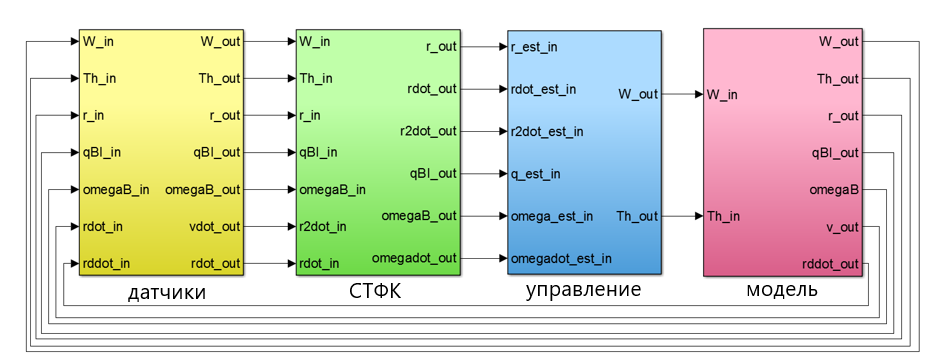
\includegraphics[width=16cm]{simulink_scheme}
	\caption{ -- Общая схема численной модели}
	\label{fig:simulink_scheme}
\end{figure}
В качестве численных методов для моделирования движения БЛА используется метод Рунге-Кутты 4-го порядка с шагом интегрирования $dt={10^{-3}}$c.

\section{Параметры управляемой динамики БЛА и соответствующие им ограничения}

Маневренные возможности любого летательного аппарата напрямую зависят от основных параметров его динамики.
Они, в свою очередь, ограничены множеством доступных для проектирования летательного аппарата подсистем, таких, как подсистема эноргообеспечения, подсистема исполнительных органов управления, вычислительная система и другие. 
В данной работе, с учетом сформулированных в разделе \ref{section_ctrl_task} задач управления, для эксперимента выбраны параметры, соответсвующие небольшому квадрокоптеру, способному нести на борту дополнительную нагрузку в виде камеры высокого разрешения и использующему в качестве источника питания малогабаритную электрическую батарею; они приведены в Таблице \ref{tb:params_table}.
\begin{table}[h!]
	\centering
	\caption{ -- Параметры модели}\label{tb:params_table} 
	\begin{tabular}{lcl}
		\hline
		Параметр & Обозначение & Значение  \\\hline
		Общая масса & $M$ & 2 кг  \\
		Тензор инерции корпуса & $\bm J_B$ & $diag(2,\ 2,\ 4)\cdot{10^{-2}}$ кг$\cdot$м$^2$  \\
		Тензор инерции ротора & $\bm J_R$ & $diag(2,\ 2,\ 1)\cdot{10^{-5}}$ кг$\cdot$м$^2$  \\
		Миделево сечение корпуса & $S_{\perp}$ & 0,12 м$^2$ \\
		Луч & $L$ & 0,25 м \\
		Аэродинамический коэффициент & $C$ & 1,05\\
		Аэродинамический коэффициент & $k$ & 1,13$\cdot 10^{-5}$ Н$\cdot$с$^2\cdot$рад$^{-2}$ \\		
		Аэродинамический коэффициент & $b$ & 1,5$\cdot 10^{-6}$ Н$\cdot$м$\cdot$с$^2\cdot$рад$^{-2}$ \\		
		Максимальные обороты & $\tilde \omega_{max}$ & 1140 рад/с \\		
		Максимальный угол & $\theta_{max}$ & ${\pi}/{3}$ рад \\
		Константа балансировки & $\varepsilon_\tau$ &6 Н$\cdot$м \\
		\hline
	\end{tabular}
\end{table}

Эти параметры использовались для рассчета ограничений на выходы регулятора \eqref{eq:m_reg} с использованим алгоритма, описанного в разделе \ref{section:limits}. Сначала было выбрано направление диагонали прямоугольной области $\Psi_{\boldsymbol{y}}$ таким образом, чтобы ограничения на выход регулятора \eqref{eq:m_reg} позволяли решать поставленные в эксперименте задачи. 
Для рассматриваемой конфигурации, описанной в Таблице \ref{tb:params_table}, выберем
$$\bm d = (0,577, 0,577, 0,577, 0,014, 0,014, 0,014).$$
Для выбранной диагонали найдем значения пределов ограничений \eqref{eq:lims_final} и балансировочных параметров, входящих в дополняющие модель \eqref{eq:m_dyn} уравнения \ref{eq:m_dyn_balance_1}, \ref{eq:m_dyn_balance_2}. Результаты приведены в Таблице \ref{tb:lims_table}.
\begin{table}[h!]
	\centering
	\caption{Параметры ограничений}\label{tb:lims_table} 
	\begin{tabular}{lcl}
		\hline	
		Длина диагонали & $2\gamma^*$ & $28$ \\
		Константа балансировки & $\varepsilon_T$ &2,6 Н$\cdot$м \\
		Константа балансировки & $\varepsilon_F$ &0 Н\\
		\hline
	\end{tabular}
\end{table}
Таким образом выполнение имеющихся ограничений параметров системы исполнительных органов управления на максимальные обороты двигателей
$\tilde \omega_{max}$ = 1140 рад/с
и на максимальные углы отклонения роторов с пропелерами от вертикали
$\theta_{max}$ = ${\pi}/{3}$ рад,
ограничивает максимально возможнок целевое ускорение БЛА по каждой из осей значением
$\ddot {\bm r}_{max}^0 \approx 4$ м/с$^2$,
угловое ускорение вдоль осей $X$ и $Y$ значением
$\dot {\bm \Omega}_{max}^0 \approx 10$ рад/с$^2$
и угловое ускорение вдоль оси $Z$ значением
$\dot {\tilde{\bm \Omega}}_{max}^0 \approx 5$ рад/с$^2$.

\section{Модель бортовых датчиков и параметры кубатурного фильтра Калмана}

Для обеспечения обратных связей в контуре управления, как было отмечено в главе \ref{chapter_estimation}, в качестве алгоритма оценки состояния был выбранкубатурный фильтр Калмана, использующий в качестве вектора состояния
\begin{equation}
\bm x = (\bm r^I, \bm v^I, q_BI, \bm \Omega^B)
\end{equation}
и соответсвующие измерения
\begin{equation}
\bm z = (\bm r^I, \bm v^I, q_BI, \bm \Omega^B).
\end{equation}
В эксперименте в качестве основы для моделирования показаний бортовых сенсоров использована реально существующая и популярная среди разработчиков мультироторных роботов бортовая система Xsens MTi-7 \cite{xsens01}.
Она содержит стандартный набор необходимых для оценки состояния БЛА подсистем, включающих себя спутниковую систему глобального позиционирования, цифровой барометрический датчик давления, трехосевые электромеханические акселерометр и гироскоп, а также магнитный компас.
Устройством предусмотрена возможность автоматической калибровки датчиков для устранения статических ошибок, которые могут возникнуть при его установке.

Измерения датчиков моделируются добавлением к результатам интегрирования уравнений движения БЛА белого гауссовского шума с параметрами, соответствующими значениям, указанным в документации устройства \cite{xsens01}.
Показания угловой скорости также содержат составляющую, отвечающую за дрейф нуля датчика угловой скорости.
Стандартные отклонения для шума измерений горизонтальной составляющей позиции, вертикальной составляющей позиции, скорости, угла тангажа, крена и рысканья приведены в таблице \ref{tb:exp_noise_params}, плотность шума измерений угловой скорости равна  
${{{\rho }}_{^{{\Omega }}}} = 7\cdot{10^{-3}}$ с$^{-1}$ $\sqrt{\text{Гц}}$,
а дрейф нуля
${{\beta }}_{^{{\Omega }}} = 3\cdot{10^{-3}}$ с$^{-1}$.
\begin{table}[h!]
	\caption{ -- Параметры шума измерений}\label{tb:exp_noise_params} 
	\centering
	\begin{tabular}{|>
			{\centering\arraybackslash}m{1.5in}|>
			{\centering\arraybackslash}m{1.5in}|}
		\hline
		${{{\sigma }}_{rx}}$& 1м \\ \hline
		${{{\sigma }}_{rz}}$& 2м \\ \hline
		${{{\sigma }}_{v}}$& 0.5м/с \\ \hline
		${{{\sigma }}_{\alpha}}$& 0.5$^\circ$ \\ \hline
		${{{\sigma }}_{\beta}}$& 0.5$^\circ$ \\ \hline
		${{{\sigma }}_{\gamma}}$& 1.5$^\circ$ \\ \hline
	\end{tabular}
\end{table}
Для выбранных датчиков были выбраны
ковариационная матрицы шума системы и шума измерений
$\bm Q$,
$\bm R$,
из выражений \eqref{eq:ukf_p_apr}, \eqref{eq:ukf_s_k}
\small
\begin{equation}
\begin{aligned}
&\bm Q = diag(1,\ 1,\ 2,\ {10^{-1}}, {10^{-1}}, {10^{-1}}, {10^{-2}}, {10^{-4}}, {10^{-4}}, {10^{-4}}, {10^{-2}}, {10^{-2}}, {10^{-2}}),
\\
&\bm R = diag({10^{-2}}, {10^{-2}}, {10^{-2}}, {10^{-2}}, {10^{-2}}, {10^{-2}}, {10^{-6}}, {10^{-6}}, {10^{-6}}, {10^{-6}}, {10^{-2}}, {10^{-2}}, {10^{-2}}).
\end{aligned}
\end{equation}
\normalsize

\section{Эксперимент: наблюдение за подвижным объектом}

В эксперименте аппарат должен выполнить наблюдение за подвижным объектом, летя неподалеку от него и ориентируя камеру, установленную спереди, так, чтобы объект находился в центре полученного изображения.
Мы не рассматриваем вопрос построения траектории БЛА, считая ее определённой заранее.
Точка старта аппарата расположена на расстоянии 90 метров от цели, затем оно постепенно сокращается до 50 метров.
Траектория БЛА и наблюдаемого объекта изображены на рисунке \ref{fig:mau_traj}.
\begin{figure}[H]
	\centering
	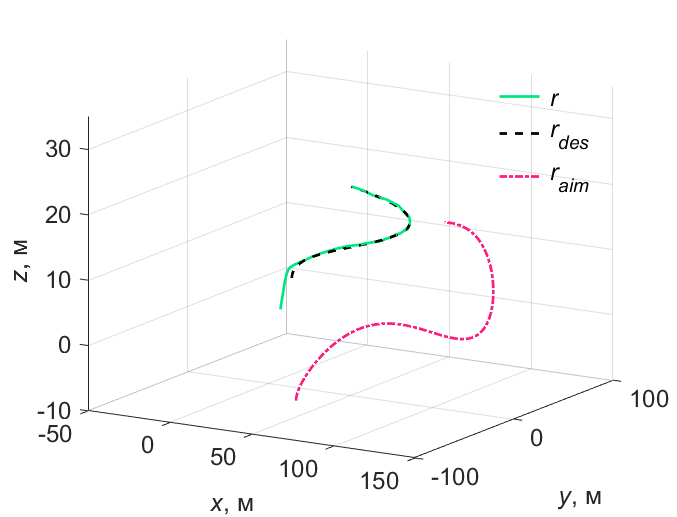
\includegraphics[width=14cm]{traj.png}
	\caption{ -- Траектория БЛА и объекта наблюдения}
	\label{fig:mau_traj}
\end{figure}

На рисунке \ref{fig:mau_errors}, на графиках слева, изображены ошибки ориентации по углам крена, тангажа и рысканья,
а справа -- ошибки положения  квадрокоптера по осям $X$, $Y$ и $Z$.
Ошибки по каждому из углов ориентации после стабилизации не превышают одного градуса.
После выхода аппарата на целевую траекторию максимальное абсолютное отклонение от траектории составило 30 см.
\begin{figure}[H]
	\centering
	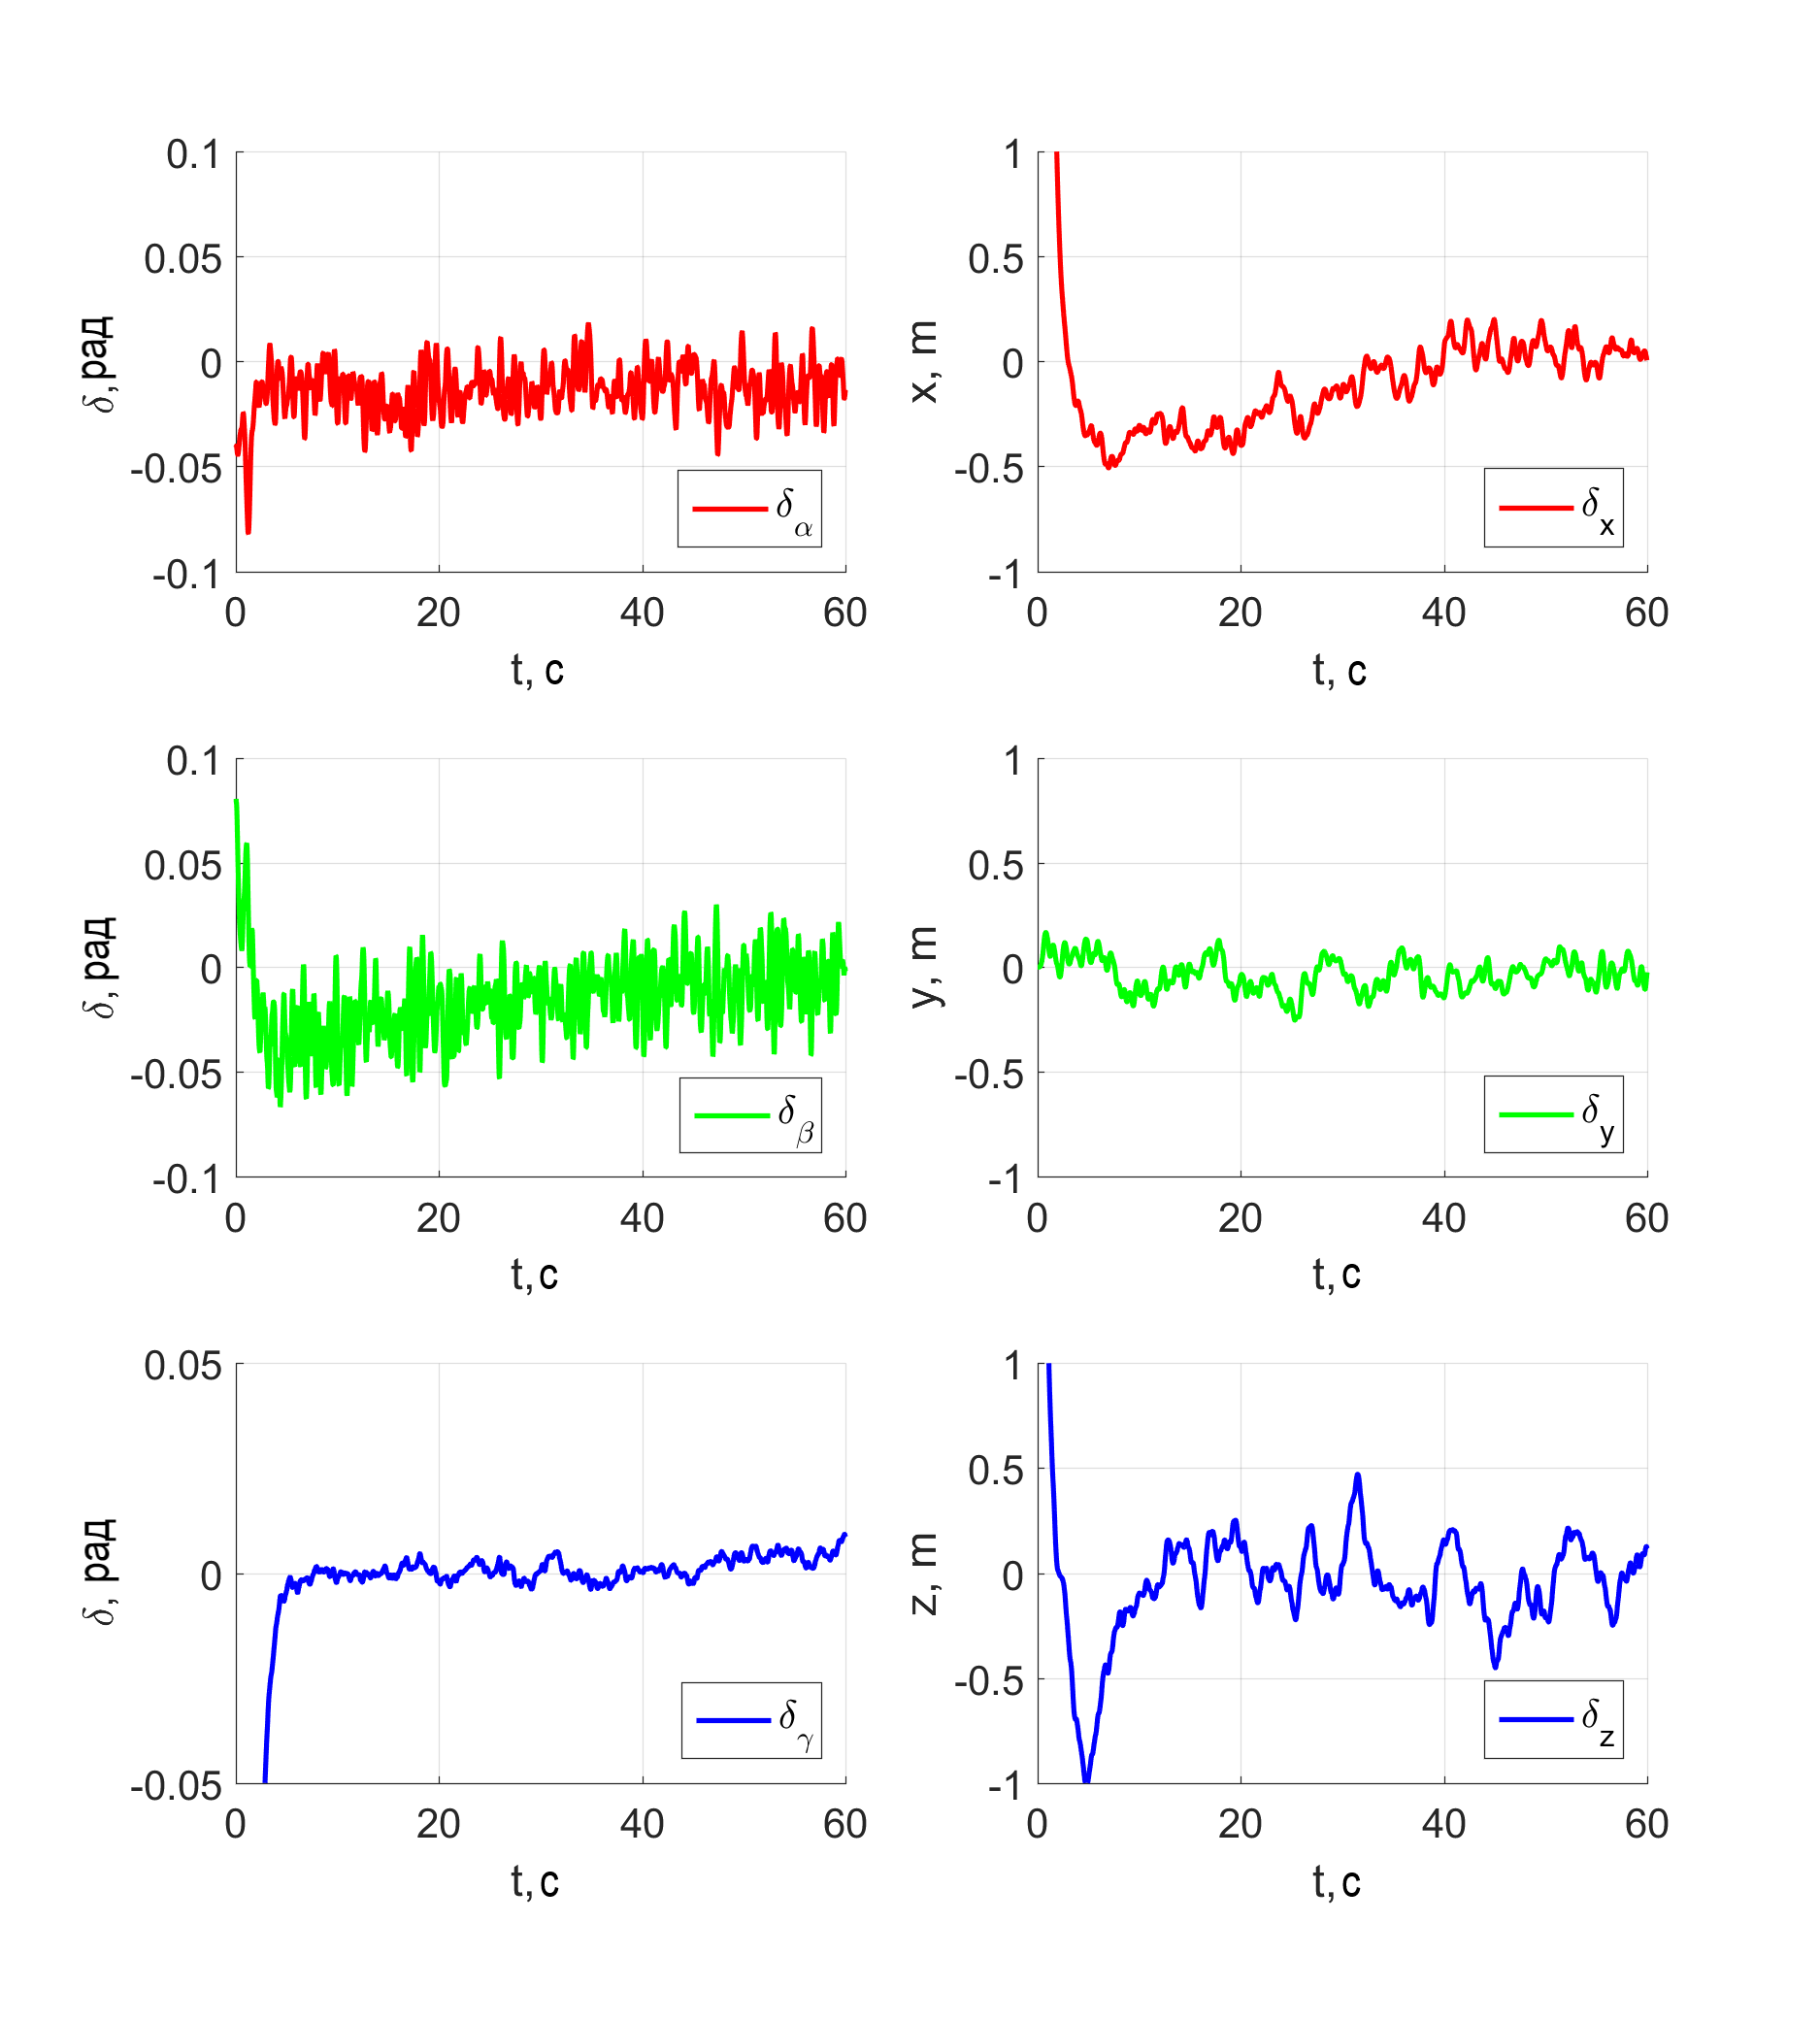
\includegraphics[width=14cm]{errors_rows.png}
	\caption{ -- Отклонение параметров движения БЛА от целевых значений}
	\label{fig:mau_errors}
\end{figure}

На рисунке \ref{fig:mau_cam} можно проследить за траекторией наблюдаемого объекта на записи, которою можно сделать с помощью передней камеры.
Видно, что в начальный момент времени объект находится вне зоны видимости, затем перемещается в центр экрана и далее на протяжении всего времени манёвра ось визирования камеры отклоняется от направления на объект не более чем на 1$^\circ$.
\begin{figure}[H]
	\centering
	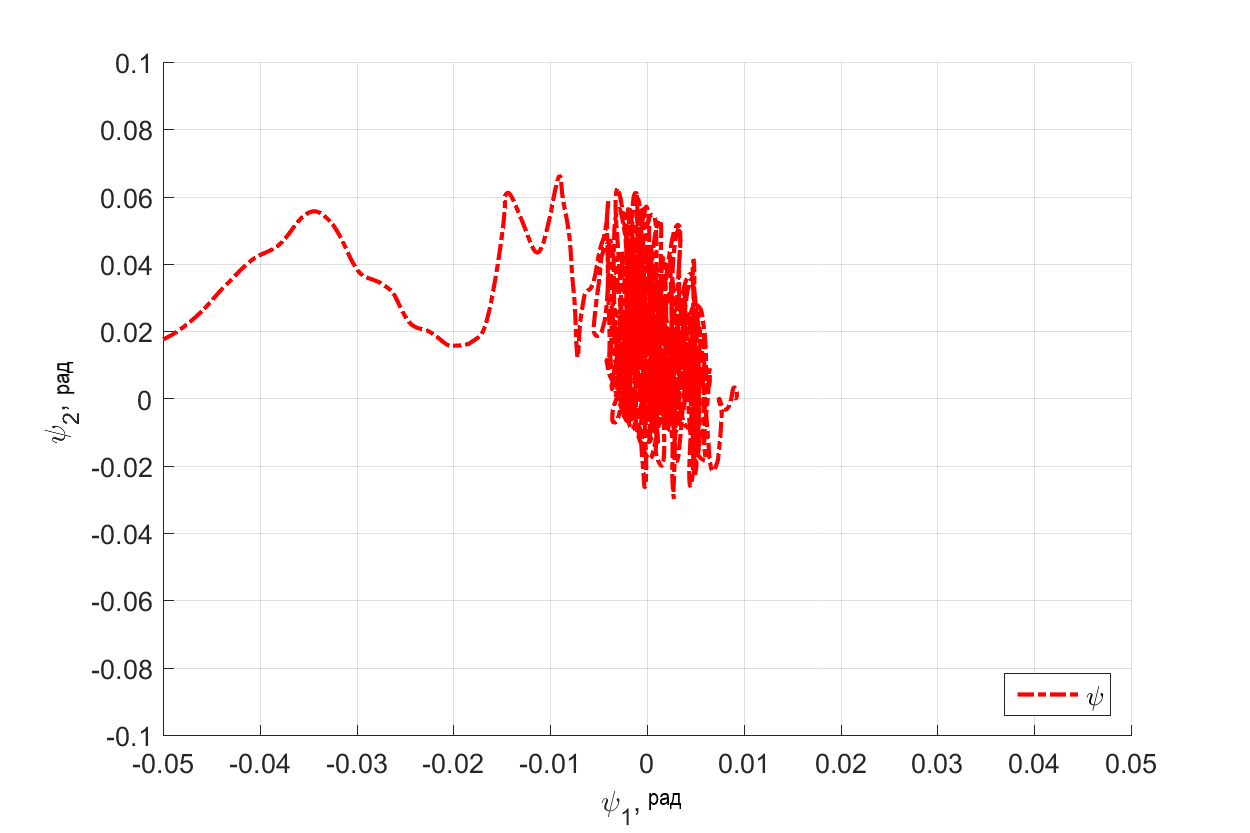
\includegraphics[width=14cm]{camera.png}
	\caption{ -- Траектория объекта на записи}
	\label{fig:mau_cam}
\end{figure}
Рисунок \ref{fig:mau_est} демонстрирует производительность алгоритмов оценки состояния. Слева приведены графики ошибки оценки углов крена, тангажа и рысканья и их прямых измерений. Справа – оценка положения по осям $X$, $Y$ и $Z$  и их прямые измерения.
\begin{figure}[H]
	\centering
	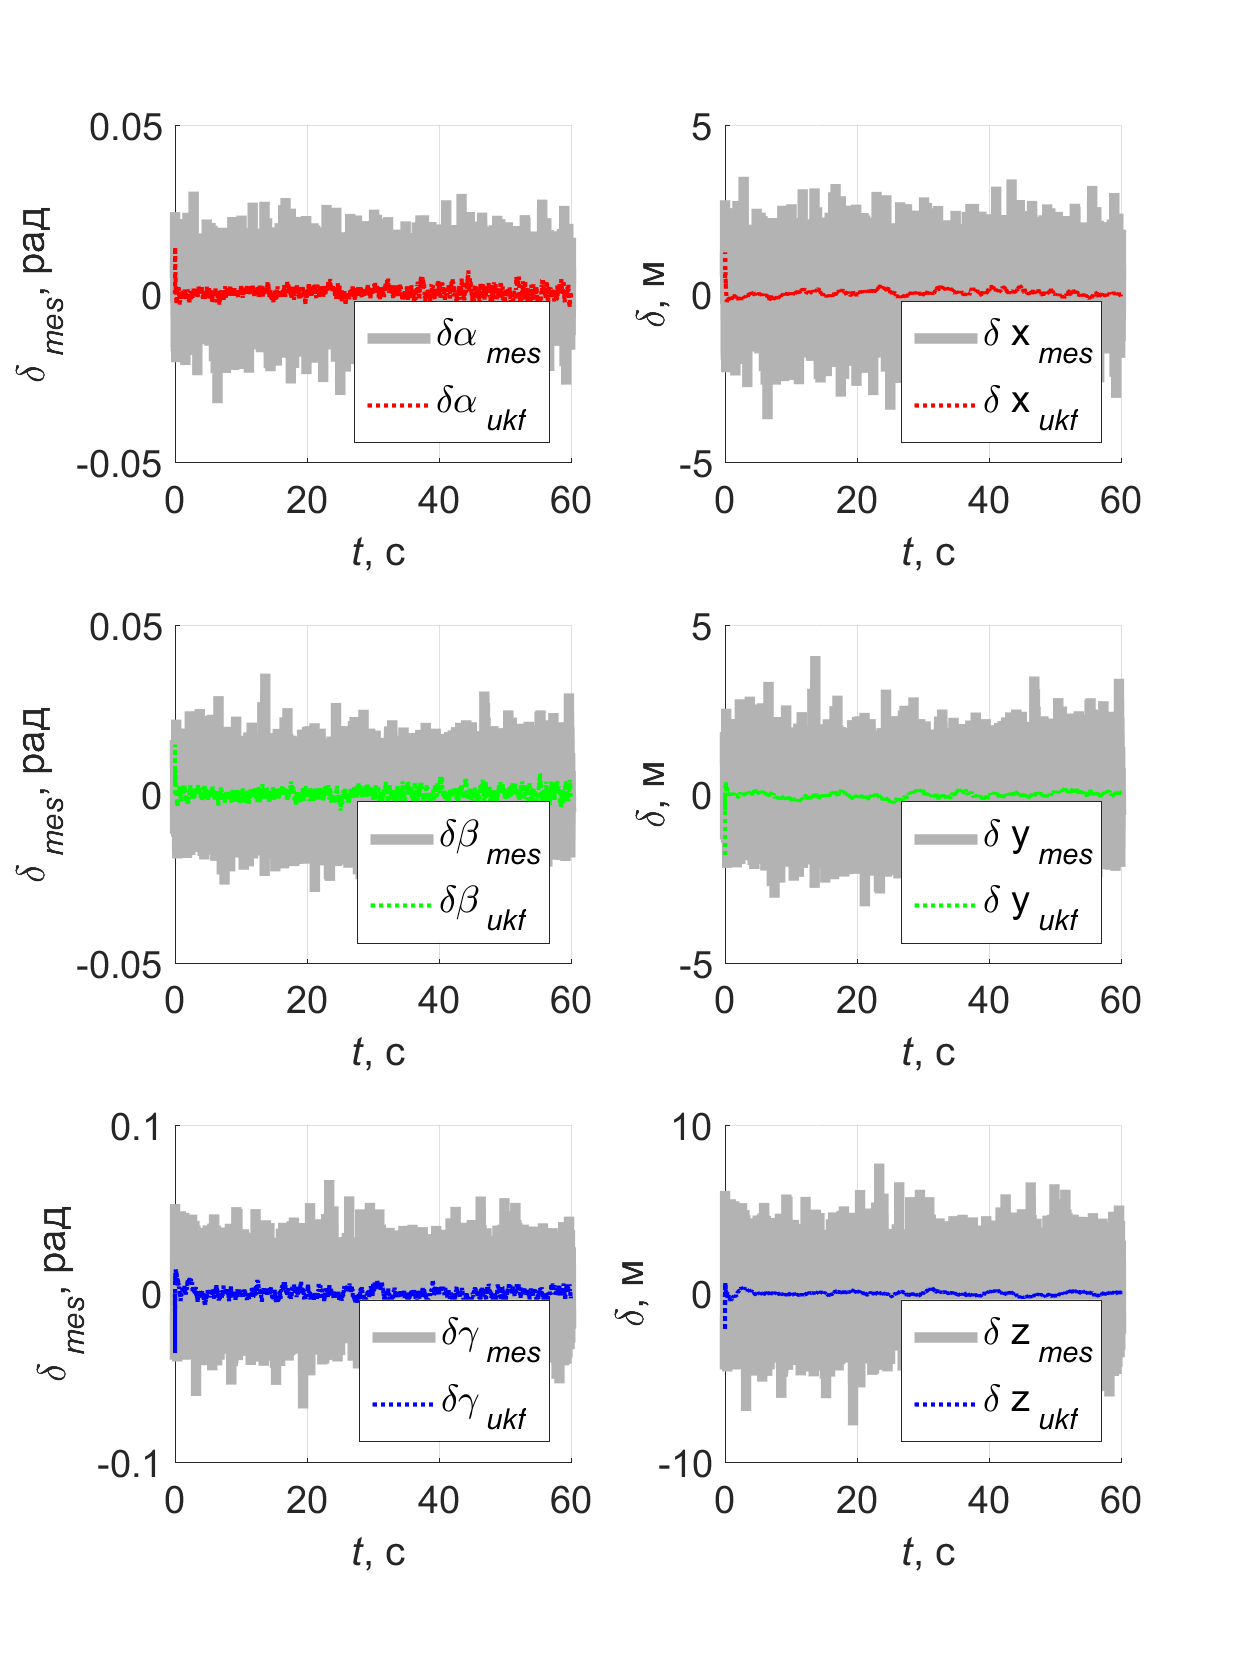
\includegraphics[width=14cm]{ukf_perf_raws.png}
	\caption{ -- Ошибка оценки состояния и прямых измерений}
	\label{fig:mau_est}
\end{figure}
Алгоритмы фильтрации позволили значительно снизить уровень шума измерений.

На графиках, изображенных на рисунке \ref{fig:mau_ctrl_out} представлены компоненты вектора управляющих параметров, которые, как легко заметить, лежат внутри ограниченной предельными значениями области.

\begin{figure}[H]
	\centering
	\subfloat{%
		\subfloat[]{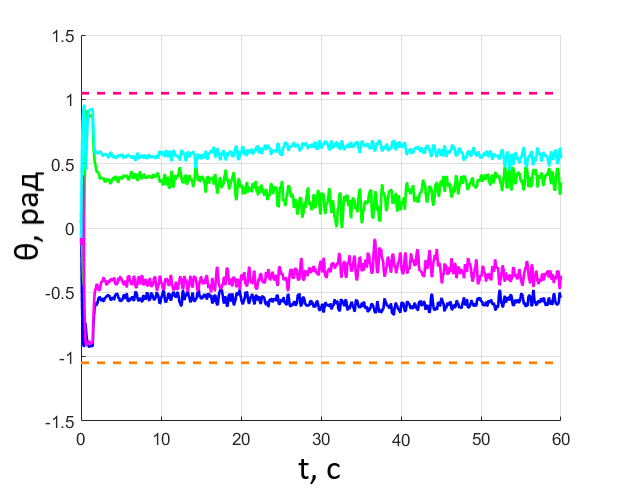
\includegraphics[clip,width=0.49\columnwidth]{rotor_angles}}%
		\subfloat[]{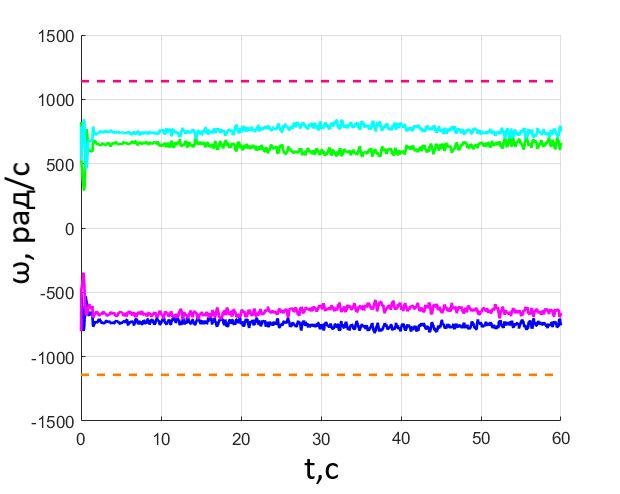
\includegraphics[clip,width=0.49\columnwidth]{rotor_rates}}%
	}
	
	\caption{ -- Управляющие параметры}
	\label{fig:mau_ctrl_out}
	
\end{figure}


В результате эксперимента мы оценили способность БЛА с поворотными роторами справляться со сложными маневрами, где необходимо независимо управлять ориентацией и положением аппарата. Квадрокоптер быстро вышел на целевую траекторию и успешно отслеживал ее, ориентируя бортовую камеру таким образом, чтобы объект наблюдения всегда оставался в центре изображения.
Стоит отметить, что при необходимости более точного отслеживания траектории имеет смысл использовать более чувствительные инструменты для измерения текущего положения и скорости, например, технологию RTK GPS \cite{Feng01}, где применение неподвижной наземной базовой станции уменьшает погрешность измерений на 1-2 порядка.


\section{Эксперимент: экстренная посадка}

В данном эксперементе рассматривается сценарий отказа двух смежных двигателей. Применяются алгоритмы управления, описанные в разделе \ref{section_em_ctrl}. Как было отмечено, для возможности применения системы экстренного управления необходим значительный запас тяги двигателей и более широкие пределы отклонений сервоприводов. Поэтому в данном эксперементе параметры ограничений БЛА несколько отличаются от тех, что представлены в таблице \ref{tb:params_table}, а именно
\begin{equation}
\begin{aligned}
&\tilde{\omega}_{max} = 1318 рад/c,
\\
&\theta_{max} = \pi.
\end{aligned}
\end{equation}

В начальный момент времени аппарат находится на высоте 25 метров недалеко от точки взлета.
При отказе двигателей начинается переход в режим экстренного управления.
За время менее 5 секунд высота БЛА упала более чем на 15 метров, но затем, когда аппарат стабилизиировал свою ориентацию около целевых значений, падение прекратилось и аппарат приступил к плавному снижению со скоростью около 0,5 метров в секунду с одновременным движением в сторону места своего запуска. По истечении 30 секунд квадрокоптер стабилизировал свое положение около точки взлета. На рисунке \ref{fig:em_coords} представлены параметры движения мультироторного робота в процессе экстренной посадки. Слева изображены графики компонент векторной части кватерниона ориентации корпуса, справа -- проекции координат центра масс БЛА на оси инерциальной системы отсчета.
\begin{figure}[H]
	
	\centering
	\subfloat[крен]{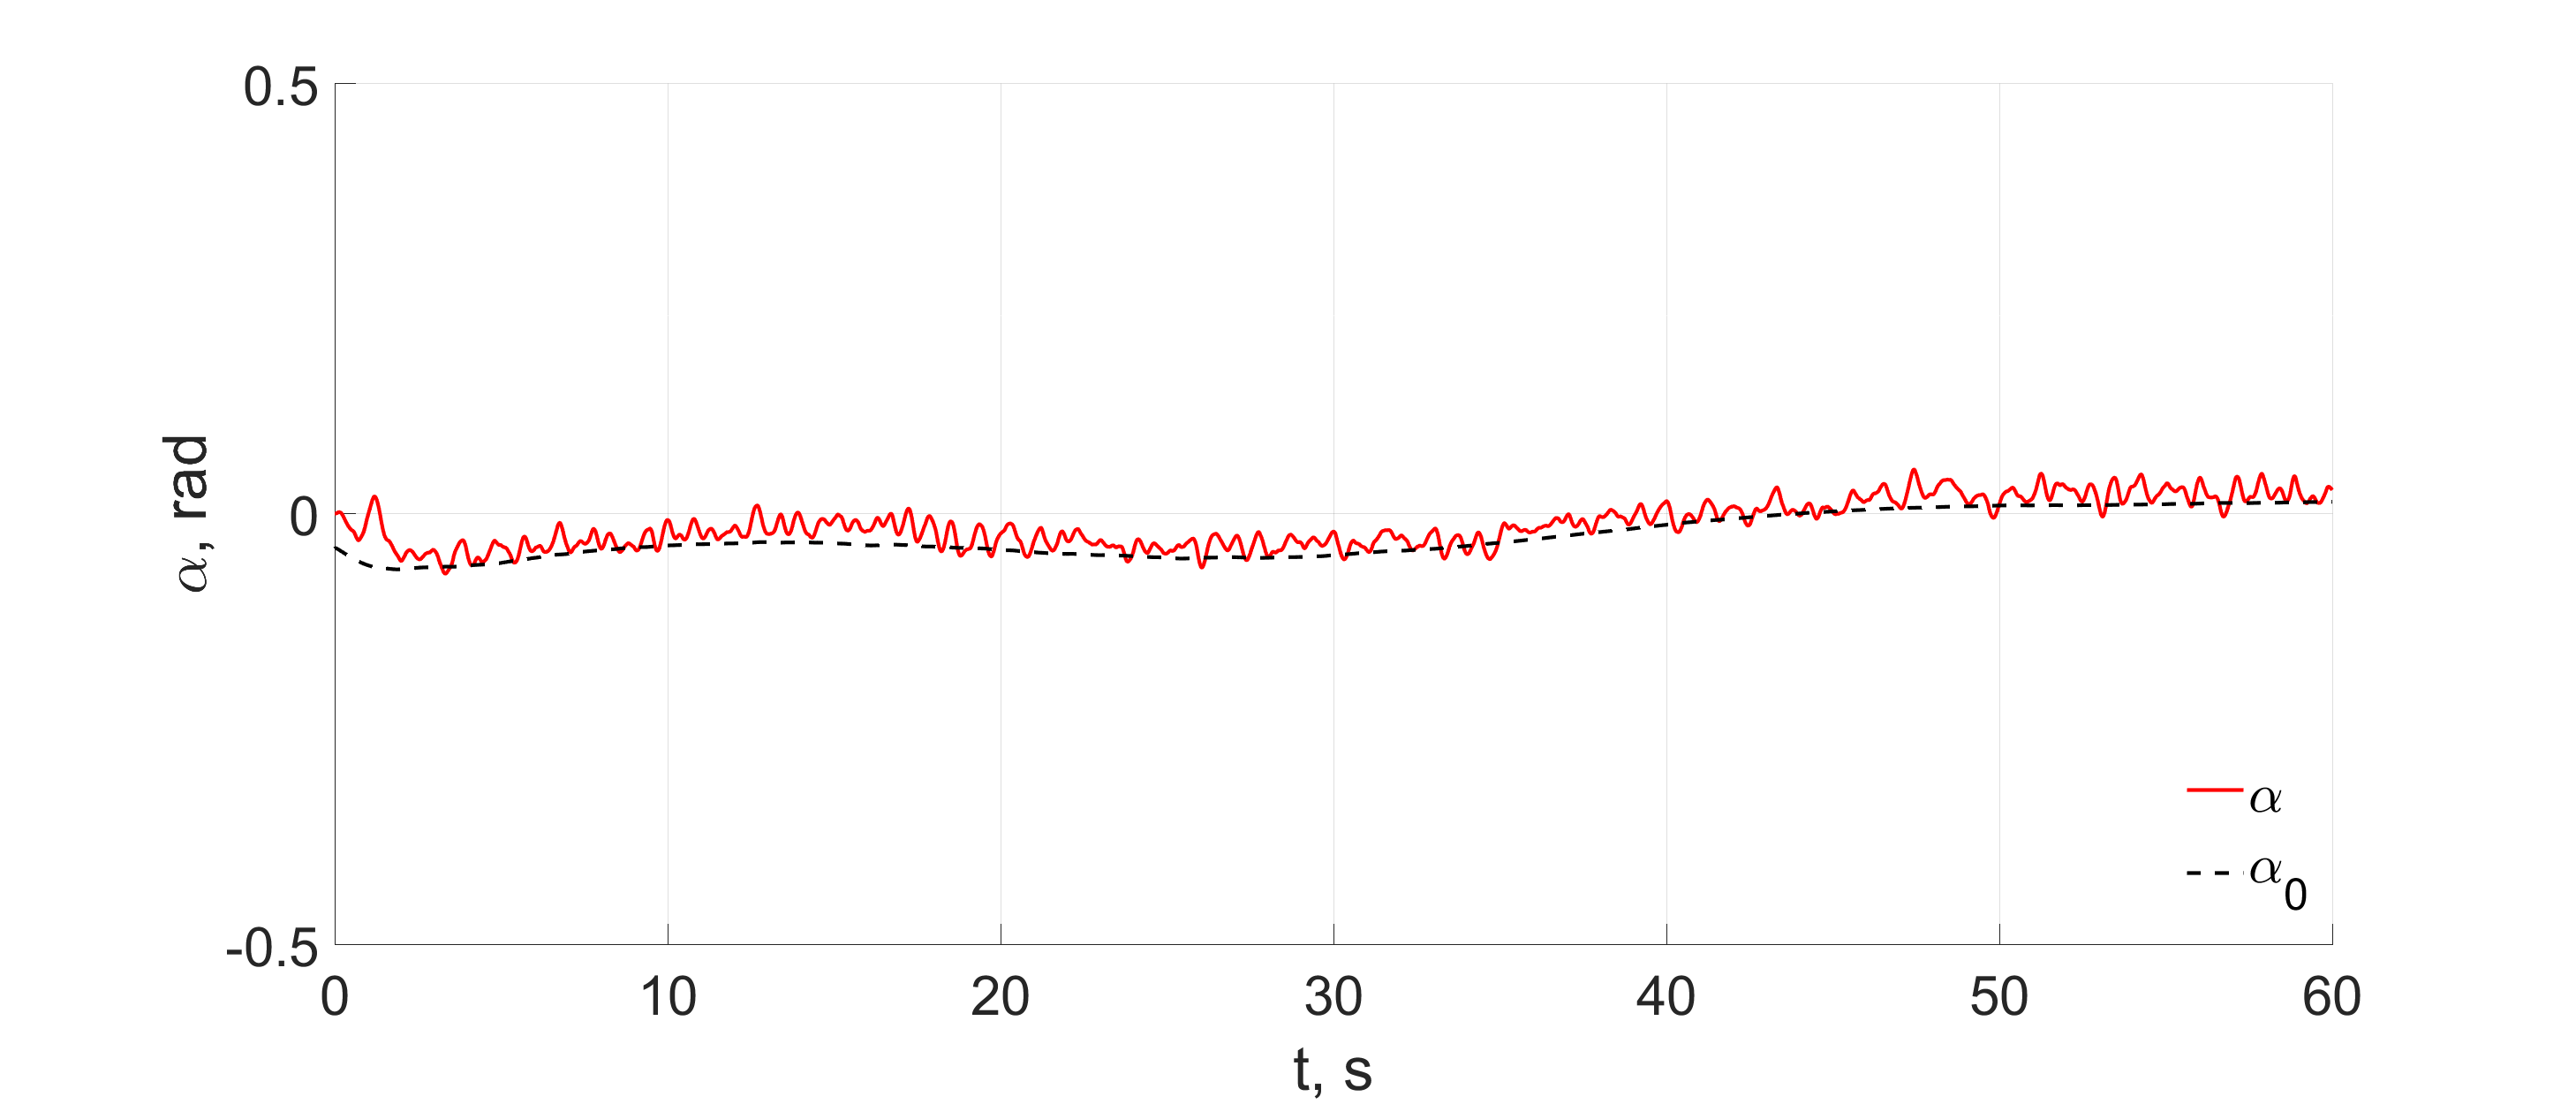
\includegraphics[width=8cm]{em/roll}}\hfil
	\subfloat[коордиата x]{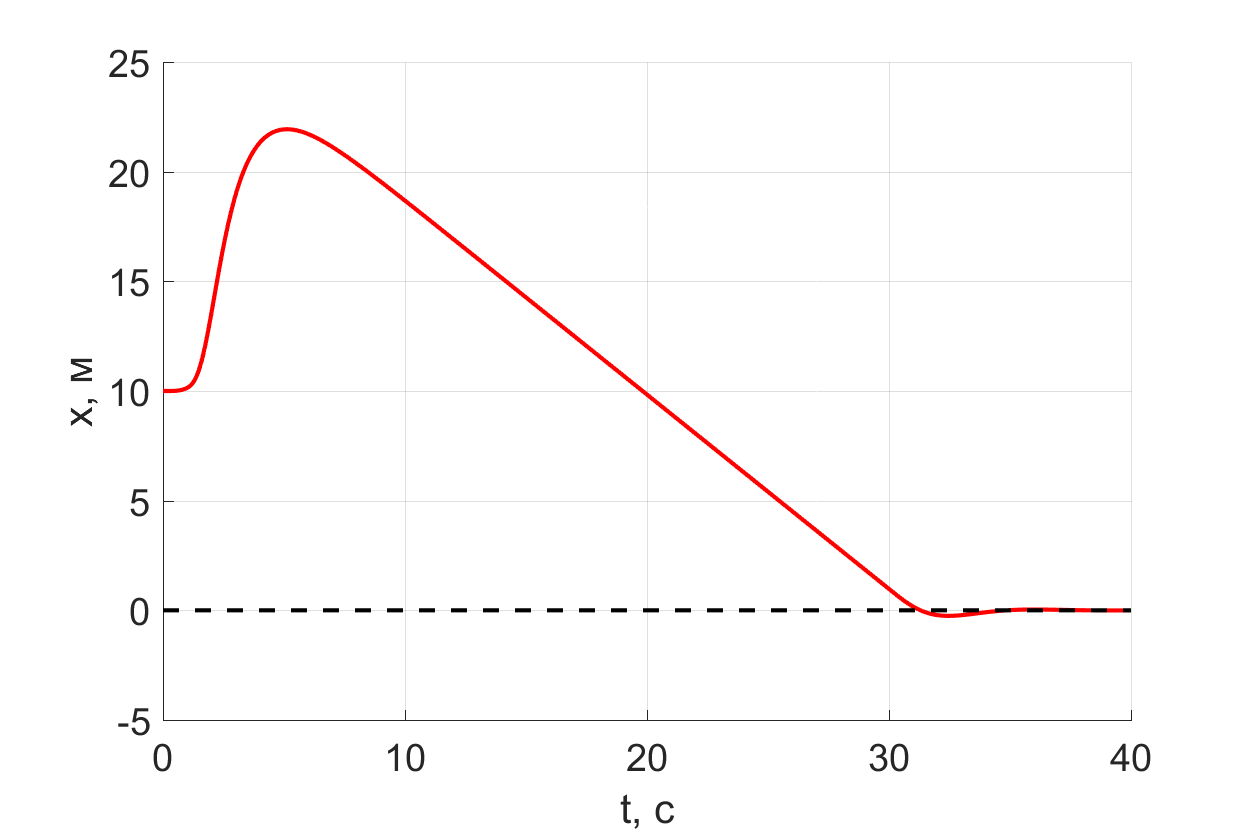
\includegraphics[width=8cm]{em/x}}
	
	\subfloat[тангаж]{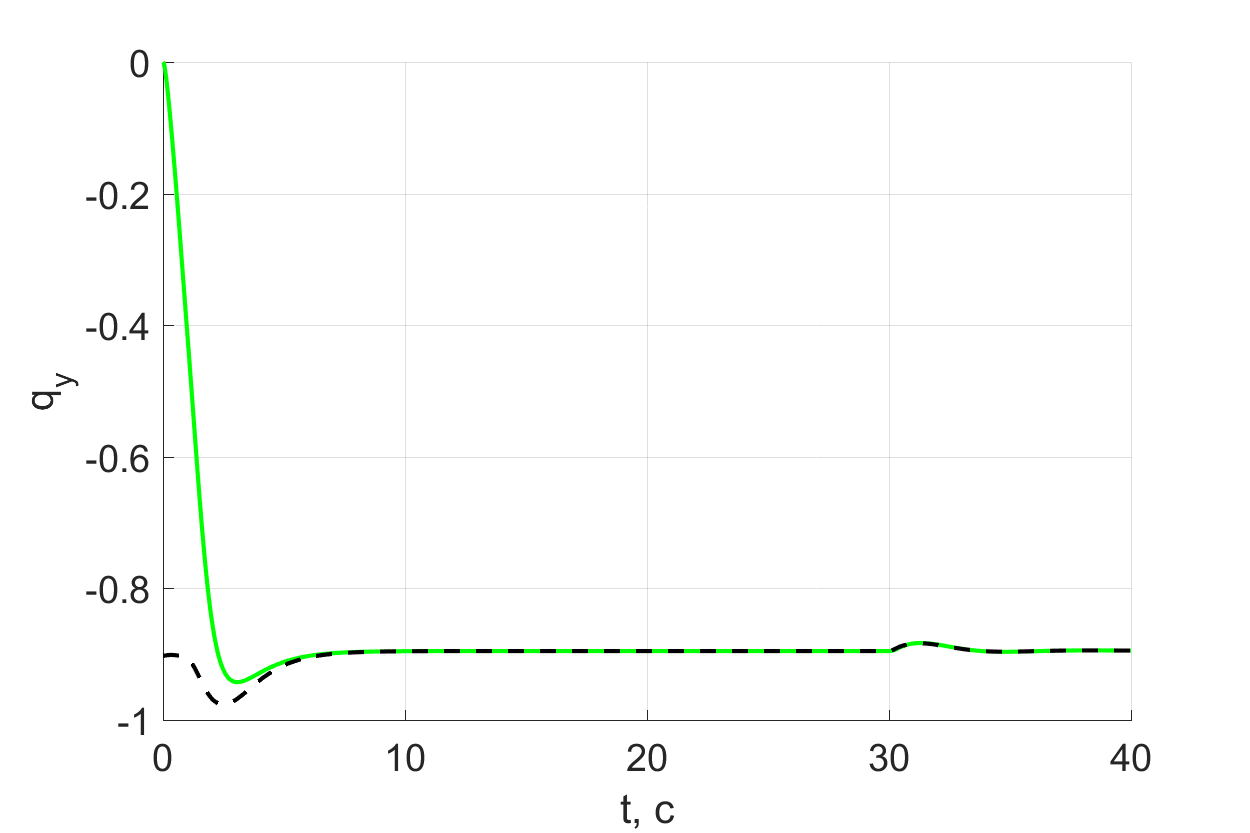
\includegraphics[width=8cm]{em/pitch}} \hfil 
	\subfloat[коордиата y]{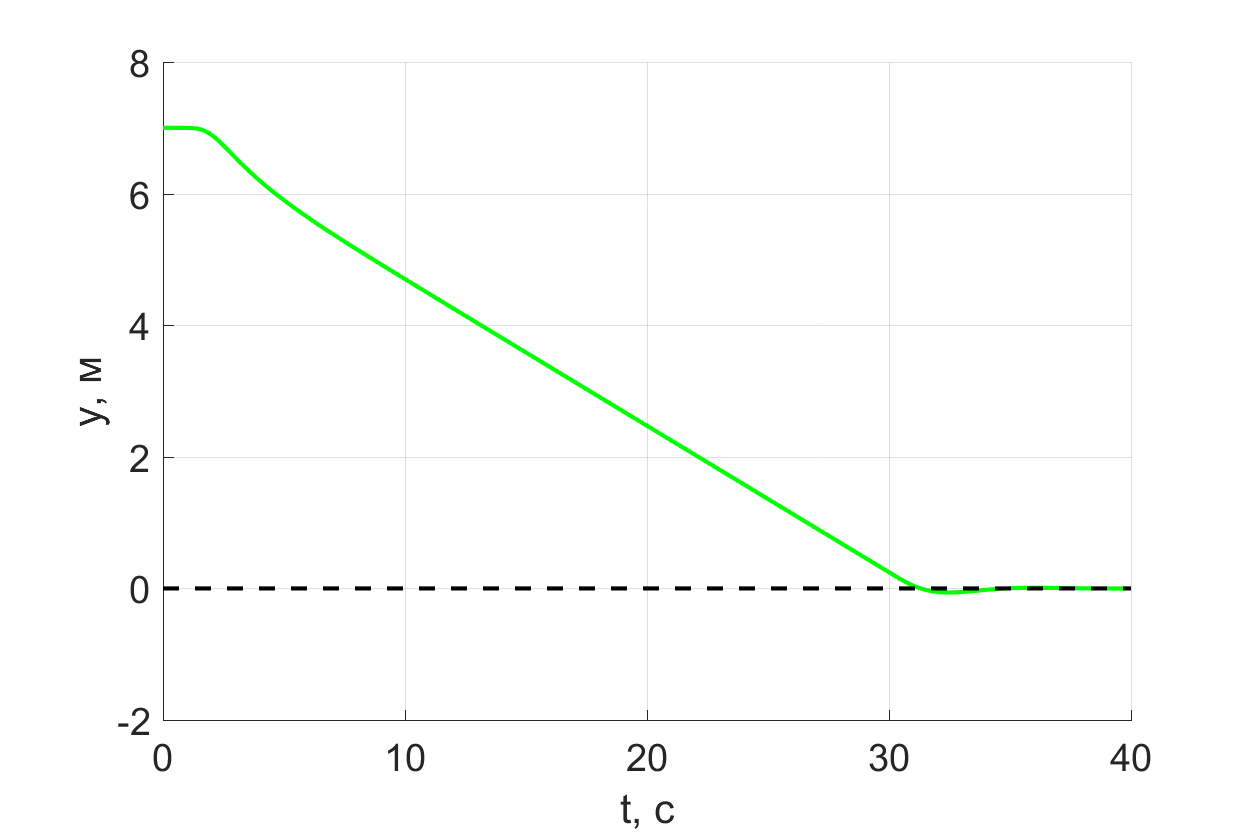
\includegraphics[width=8cm]{em/y}}  
	
	\subfloat[рысканье]{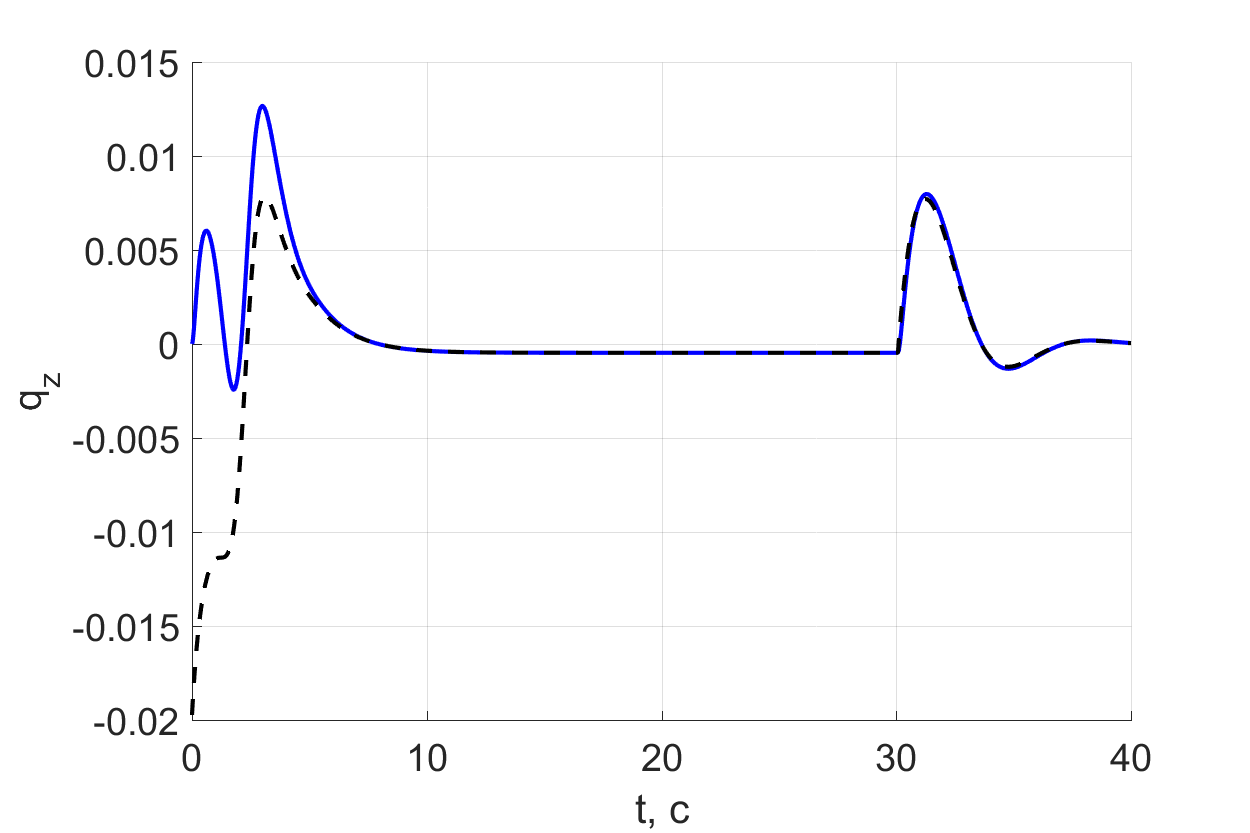
\includegraphics[width=8cm]{em/yaw}}\hfil
	\subfloat[коордиата z]{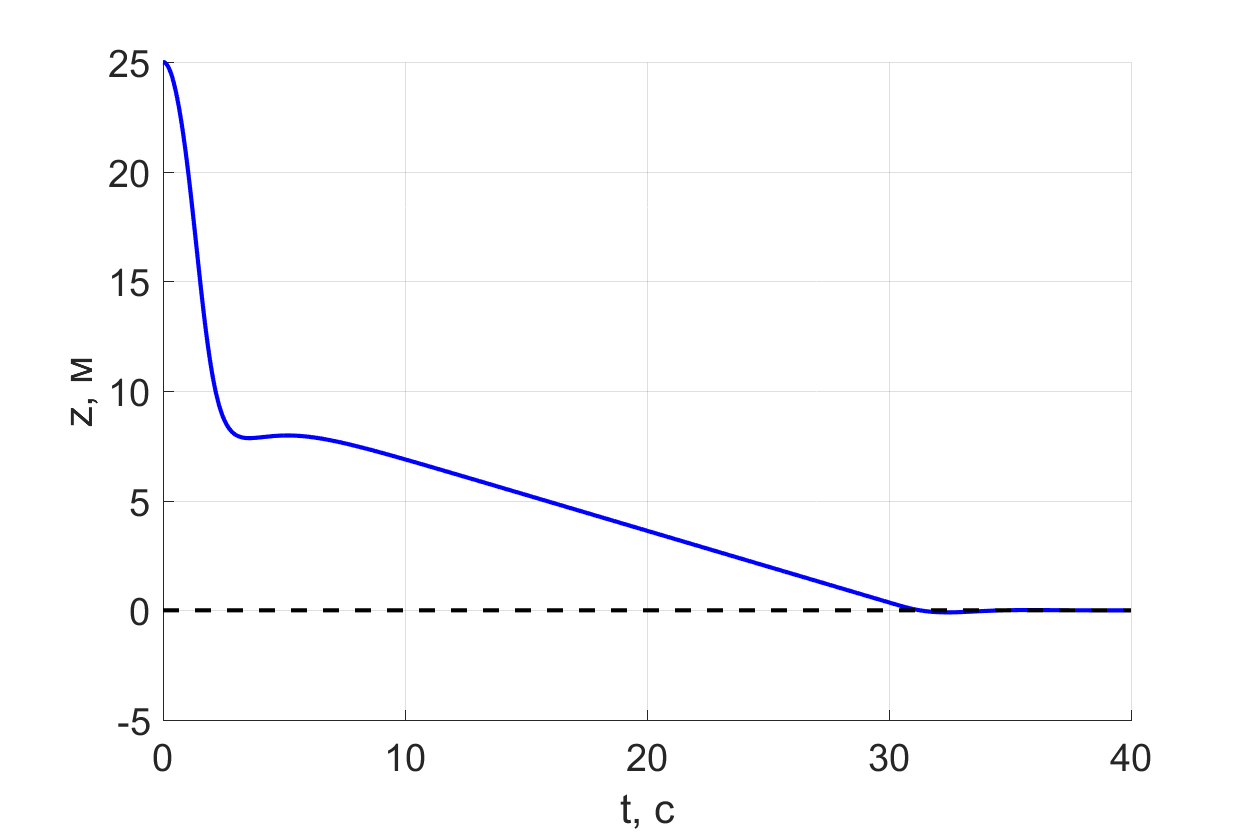
\includegraphics[width=8cm]{em/z}}
	\caption{ -- Параметры движения БЛА при экстренной посадке}
	\label{fig:em_coords}
\end{figure}

Таким образом было показано, что БЛА с поворотными роторами при соблюдении некоторых требований к параметрам исполнительных органов системы управления способен продолжить свое движение после отказа двух смежных двигателей.